\chapter{Results and Analysis}
\label{results}

This chapter details the results of tuning and evaluating the CGT model. All available user-item ratings were used to tune the rating model, while 90\% of the movie genre labels were used to train and tune the genre model. Only the "drama" label was used in the MovieLens datasets, as it was the most evenly balanced class. Goodbooks-10k used only the "adult-fiction" label, which had very close to 50/50 class weighting. The chapter concludes with an exploratory analysis of the item latent factors.

\section{Hyperparameter grid search}
A number of grid searches were performed to tune the hyperparameters of the CGT model. Due to the different sizes of the MovieLens (ML) datasets, the smallest dataset, ML100k, was used to test the widest range of hyperparameters. Then, a subset of the best-performing hyperparameters were tested again on the ML1M dataset. No hyperparameter tuning was done on ML10M due to its size. The best hyperparameters from ML1M were used for ML10M and GB10k.

In each grid search, the best parameters were chosen as those which minimised the average CV log loss of the genre classifications.

When initialising weights of each model, the same random seed was used to allow for reproducible results.

\subsection{MovieLens100k}
Four grid searches were performed on the ML100k dataset. The first grid search tested various combinations of $k$ -- the number of latent factors, $h$ -- the number of hidden nodes in the rating model, and $j$ -- the number of hidden nodes in the genre model. The second grid search tested different numbers of training epochs and the third tested different values of $dr1$ and $dr2$ -- the dropout rate in the hidden layers of each model. Finally, a number of different activation functions were tested. Each successive hyperparameter search used the best set of hyperparameters from the previous.

\subsubsection{Number of latent factors and hidden neurons}
Values between 50 and 200 were tested for $k$, while $h$ and $j$ were tested in the range of 25 and 100. While tuning these parameters, the dropout rate of the hidden layers, $dr1$ and $dr2$ were both fixed at 0.2 and ReLU was used as the activation function. A total of 12 different combinations were tested in this grid search, the top 5 models are shown in table \ref{tab:ml100k-grid-results1}.

\begin{table}[H]
\centering
\begin{tabular}{c | c | c | c | c}
\toprule
\textbf{$k$} & \textbf{$h$} & \textbf{$j$} & \textbf{Avg. CV log loss} & \textbf{Avg. CV acc.} \% \\
\midrule
200 & 100 & 100 & 0.6344 & 63.12 \\
\midrule
200 & 100 & 50 & 0.6365 & 62.52 \\
\midrule
100 & 100 & 100 & 0.6391 & 62.79 \\
\midrule
100 & 50 & 100 & 0.6394 & 62.39 \\
\midrule
200 & 50 & 100 & 0.6406 & 62.85 \\
\bottomrule
\end{tabular}
\caption[MovieLens 100k grid search results -- number of nodes]{Results of first grid search performed on ML100k. Average CV log loss and accuracy are shown for different combinations of $k$, $h$ and $j$.}
\label{tab:ml100k-grid-results1}
\end{table}

The best performing set of hyperparameters in the first grid search was $k=200$, $h=100$ and $j=100$. All of the top five used a latent factor vector size of either 100 or 200. All top three models had a value of 100 for $h$, while four of the top five had a value of 100 for $j$. The relationship between the size of $k$ and the average CV loss is shown in figure \ref{fig:5-latent-size}

\begin{figure}[H]
\centering
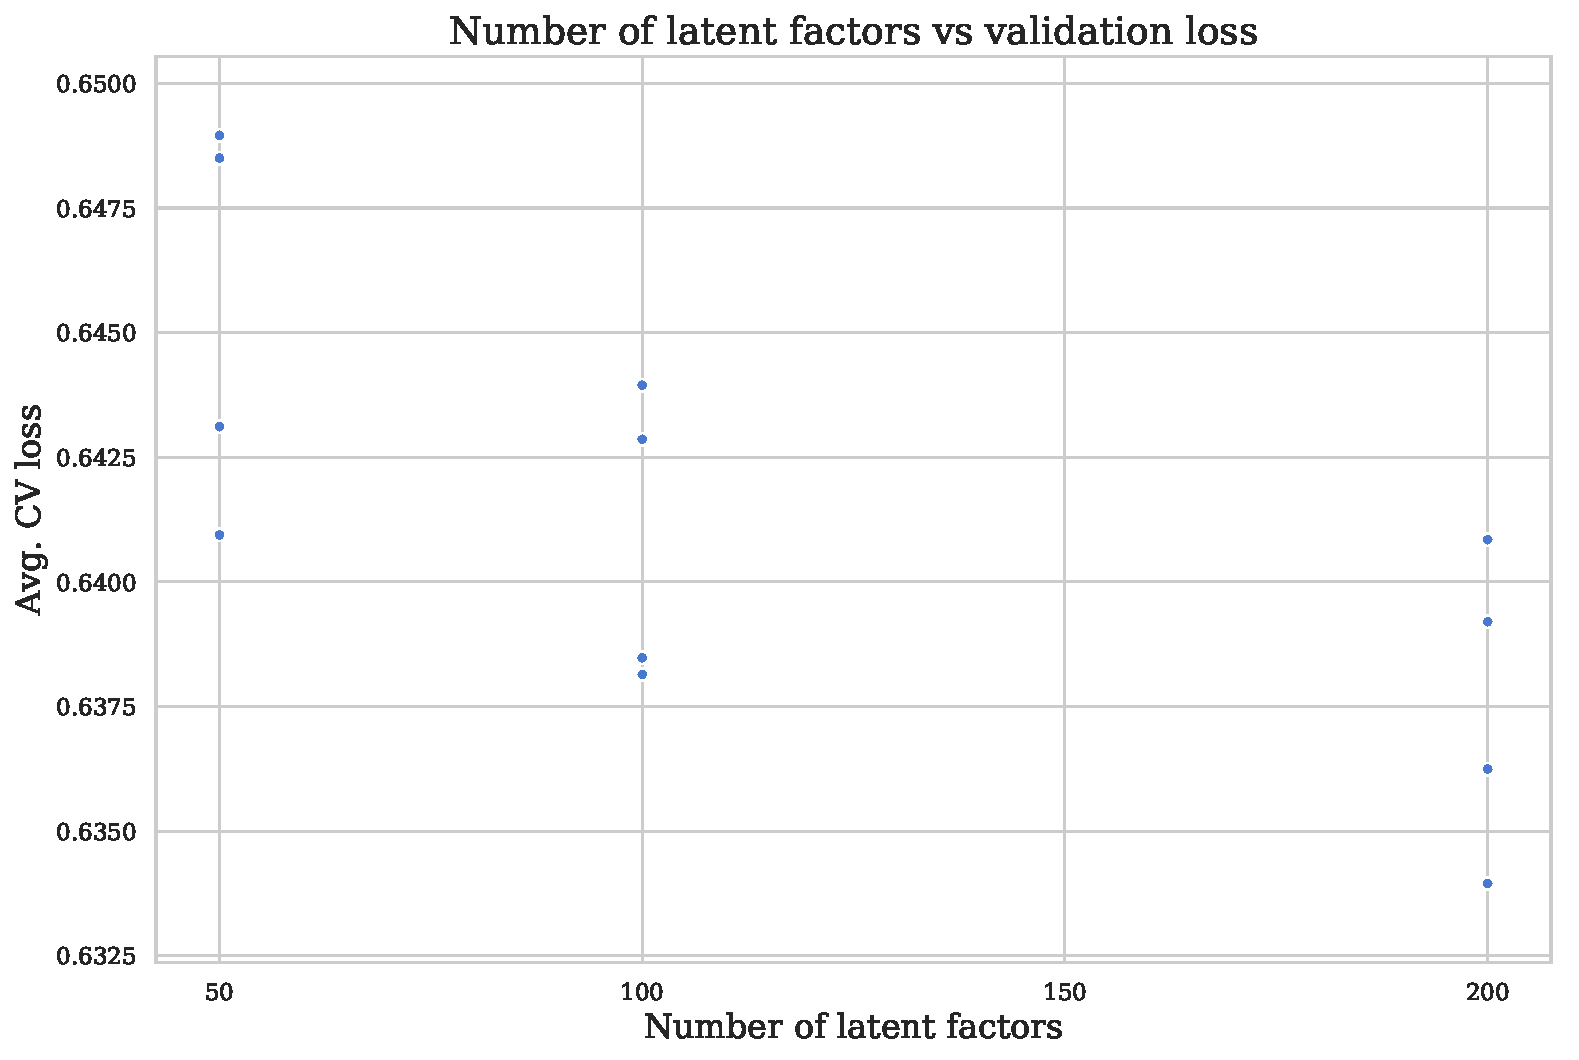
\includegraphics[width=0.78\textwidth]{Figures/5_ml100k-latent-factors.pdf}
\decoRule
\caption[Number of latent factors vs classification accuracy]{Relationship between number of latent factors and classification performance.}
\label{fig:5-latent-size}
\end{figure}

\subsubsection{Number of epochs}
Training the model for too many epochs could risk overfitting. Therefore, it was necessary to find the optimal number of epochs for both the rating and genre model. Values of 5, 6 and 7 were tested for the rating model, while values of 3, 4 and 5 were tested for the genre model. This meant a total of 9 different combinations were tested in this grid search, with each one using the hyperparameters $k$, $h$ and $j$ from the best performing model in the first grid search. The top 5 models are shown in table \ref{tab:ml100k-grid-results2}. $E1$ and $E2$ are the number of epochs used for the rating and genre model respectively.

\begin{table}[H]
\centering
\begin{tabular}{c | c | c | c}
\toprule
\textbf{$E1$} & \textbf{$E2$} & \textbf{Avg. CV log loss} & \textbf{Avg. CV acc.} \% \\
\midrule
7 & 5 & 0.6344 & 63.12 \\
\midrule
6 & 5 & 0.6353 & 63.19 \\
\midrule
7 & 4 & 0.6360 & 63.12 \\
\midrule
6 & 4 & 0.6366 & 63.32 \\
\midrule
5 & 5 & 0.6376 & 62.72 \\
\bottomrule
\end{tabular}
\caption[MovieLens 100k grid search results -- number of epochs]{Results of third ML100k grid search which tested  different combinations of $E1$ and $E2$.}
\label{tab:ml100k-grid-results2}
\end{table}

\subsubsection{Dropout rates}
The third grid search tested different combinations of dropout rates used in the hidden layers of the two models. Values between 0.15 and 0.25 were tested. A total of 9 different combinations were tested in this grid search. The top 5 models from the third grid search are shown in table \ref{tab:ml100k-grid-results3}.

\begin{table}[H]
\centering
\begin{tabular}{c | c | c | c | c}
\toprule
\textbf{$dr1$} & \textbf{$dr2$} & \textbf{Avg. CV log loss} & \textbf{Avg. CV acc.} \% \\
\midrule
0.25 & 0.15 & 0.6334 & 62.99 \\
\midrule
0.25 & 0.2 & 0.6336 & 63.32 \\
\midrule
0.25 & 0.25 & 0.6337 & 63.19 \\
\midrule
0.2 & 0.15 & 0.6343 & 63.05 \\
\midrule
0.2 & 0.2 & 0.6344 & 63.12 \\
\bottomrule
\end{tabular}
\caption[MovieLens 100k grid search results -- dropout rates]{Results of third ML100k grid search which tested different combinations of $dr1$ and $dr2$.}
\label{tab:ml100k-grid-results3}
\end{table}

The best performing model used a higher dropout rate of 0.25 in the rating model, compared to 0.15 in the genre model.

\subsubsection{Activation function}
Finally, five different activation functions were tested using the best parameters from the first three grid searches. The five activation functions used were:
\begin{itemize}
    \item Linear
    \item Rectified Linear Unit (ReLU)
    \item Scaled Exponential Linear Unit (SELU)
    \item Softplus
    \item Hyperbolic tangent (Tanh)
\end{itemize}
The CV performance of each activation function is shown in \ref{tab:ml100k-activations}.

\begin{table}[H]
\centering
\begin{tabular}{c | c | c | c | c}
\toprule
\textbf{Activation function} & \textbf{Avg. CV log loss} & \textbf{Avg. CV acc.} \% \\
\midrule
ReLU & 0.6334 & 63.12 \\
\midrule
Softplus & 0.6461 & 60.81 \\
\midrule
SELU & 0.6467 & 60.67 \\
\midrule
Tanh & 0.6494 & 59.95 \\
\midrule
Linear & 0.6500 & 59.42 \\
\bottomrule
\end{tabular}
\caption[MovieLens 100k grid search results -- activation function]{Comparison of activation functions}
\label{tab:ml100k-activations}
\end{table}

\subsection{MovieLens1M}
A second set of grid searches was performed on MovieLens1M, using a subset of the best performing values tested on MovieLens100k. The parameters tested on ML1M included the number of latent factors, number of hidden neurons, number of training epochs, and the dropout rates. The ReLU activation function was chosen for this dataset, as it was significantly better than the other four that were tested on ML100k.

\subsubsection{Number of latent factors and hidden neurons}
Values of 100 and 200 were tested for $k$, while $h$ and $j$ were tested between 50 and 100. This totalled 8 different combinations, of which the top 5 models are shown in table \ref{tab:ml1m-grid-results1}.

\begin{table}[H]
\centering
\begin{tabular}{c | c | c | c | c}
\toprule
\textbf{$k$} & \textbf{$h$} & \textbf{$j$} & \textbf{Avg. CV log loss} & \textbf{Avg. CV acc.} \% \\
\midrule
200 & 100 & 100 & 0.5815 & 69.00 \\
\midrule
200 & 100 & 50 & 0.5947 & 67.92 \\
\midrule
200 & 50 & 100 & 0.5997 & 66.78 \\
\midrule
100 & 100 & 100 & 0.6013 & 66.33 \\
\midrule
200 & 50 & 50 & 0.6058 & 66.00 \\
\bottomrule
\end{tabular}
\caption[MovieLens 1M grid search results -- number of nodes]{Best values of $k$, $h$ and $j$ on MovieLens 1M dataset.}
\label{tab:ml1m-grid-results1}
\end{table}

As was the case with ML100k, the best values for $k$, $h$ and $j$ for ML1M were 200, 100 and 100 respectively.

\subsubsection{Number of epochs}
Values of 7 and 8 were tested for $E1$ and 5, 6 and 7 were tested for $E2$. The top 5 combinations of $E1$ and $E2$ are shown in table \ref{tab:ml1m-grid-results2}.

\begin{table}[H]
\centering
\begin{tabular}{c | c | c | c}
\toprule
\textbf{$E1$} & \textbf{$E2$} & \textbf{Avg. CV log loss} & \textbf{Avg. CV acc.} \% \\
\midrule
8 & 7 & 0.5714 & 69.12 \\
\midrule
8 & 6 & 0.5728 & 69.50 \\
\midrule
8 & 5 & 0.5761 & 69.92 \\
\midrule
7 & 7 & 0.5767 & 68.86 \\
\midrule
7 & 6 & 0.5783 & 68.94 \\
\bottomrule
\end{tabular}
\caption[MovieLens 1M grid search results -- number of epochs]{Number of training epochs for both models on ML1M.}
\label{tab:ml1m-grid-results2}
\end{table}

\subsubsection{Dropout rates}
The same values of $d1$ and $d2$ that were tested on ML 100k were tested again on this dataset, the results are shown below in table \ref{tab:ml1m-grid-results3}.

\begin{table}[H]
\centering
\begin{tabular}{c | c | c | c | c}
\toprule
\textbf{$dr1$} & \textbf{$dr2$} & \textbf{Avg. CV log loss} & \textbf{Avg. CV acc.} \% \\
\midrule
0.15 & 0.15 & 0.5664 & 69.69 \\
\midrule
0.15 & 0.2 & 0.5665 & 69.63 \\
\midrule
0.15 & 0.25 & 0.5668 & 69.81 \\
\midrule
0.25 & 0.15 & 0.5693 & 70.49 \\
\midrule
0.25 & 0.2 & 0.5695 & 70.37 \\
\bottomrule
\end{tabular}
\caption[MovieLens 1M grid search results -- dropout rates]{Best 5 dropout rates on MovieLens 1M dataset.}
\label{tab:ml1m-grid-results3}
\end{table}

Unlike the ML100k grid search, lower dropout rates yielded the lowest CV loss on ML1M. A value of 0.15 used as the dropout rate in both the rating and genre model resulted in the best performing model.

\section{Holdout testing}
After tuning hyperparemeters, CGT was tested against the 10\% holdout set for each of the three MovieLens datasets and the Goodbooks-10k dataset. For ML10M and Goodbooks-10k, the model was trained on 90\% of the data, using the best hyperparameters from the ML1M model, i.e. without tuning any hyperparameters.

\subsection{Classification metrics}
Performance on the holdout set was evaluated using four different classification metrics, namely accuracy, precision, recall and F1 score. The test results are shown in table \ref{tab:ml-test-results} below for all four datasets. Class weight refers to the number of movies in the holdout set which had a positive class label. For example, the holdout set in ML100k consisted of a total of 169 movies, of which 73 were dramas. 495 of the 1000 books in the Goodbooks-10k dataset had the "adult-fiction" label.

\begin{table}[H]
\centering
\begin{tabular}{c | c | c | c | c | c | c}
\toprule
\textbf{Dataset} & \textbf{Class weight} & \textbf{Accuracy} & \textbf{Precision} & \textbf{Recall} & \textbf{F1 score} \\
\midrule
ML 100k & 73/169 (43\%) & 0.63 & 0.58 & 0.52 & 0.55 \\
\midrule
ML 1M & 144/371 (39\%) & 0.70 & 0.61 & 0.61 & 0.61 \\
\midrule
ML 10M & 517/1068 (48\%) & 0.70 & 0.68 & 0.70 & 0.69 \\
\midrule
GB 10k & 495/1000 (50\%) & 0.63 & 0.63 & 0.59 & 0.61 \\
\bottomrule
\end{tabular}
\caption[Holdout classification report]{Classification performance of CGT.}
\label{tab:ml-test-results}
\end{table}

One can see above that the classification accuracy increases with the size of the dataset. ML 100k has the worst performance with 63\% of the movies correctly labelled. ML 10M, which also has the most even split between positive and negative labels (drama vs not drama), has the best performance with 70\% accuracy and an F1 score of 0.69.

\subsection{Confusion matrices}
To further break down the performance of the genre prediction, confusion matrices show the relationship between predicted and actual labels for the movies. The confusion matrices for each data set are given in tables \ref{tab:ml100k-confusion-matrix}, \ref{tab:ml1m-confusion-matrix}, \ref{tab:ml10m-confusion-matrix} and \ref{tab:gb10k-confusion-matrix} below. In each matrix, the columns represent the predicted labels and the rows represent the actual labels.

\begin{table}[H]
\centering
\begin{tabular}{c | c | c | c}
\toprule
 & \textbf{Negative} & \textbf{Positive} & \textbf{Total} \\
\midrule
\textbf{Negative} & 68 & 28 & 96 \\
\midrule
\textbf{Positive} & 35 & 38 & 73 \\
\midrule
\textbf{Total} & 103 & 66 & 169 \\
\bottomrule
\end{tabular}
\caption[MovieLens 100k confusion matrix]{Confusion matrix of ML100k holdout set.}
\label{tab:ml100k-confusion-matrix}
\end{table}

\begin{table}[H]
\centering
\begin{tabular}{c | c | c | c}
\toprule
 & \textbf{Negative} & \textbf{Positive} & \textbf{Total} \\
\midrule
\textbf{Negative} & 170 & 57 & 227 \\
\midrule
\textbf{Positive} & 56 & 88 & 144 \\
\midrule
\textbf{Total} & 226 & 145 & 371 \\
\bottomrule
\end{tabular}
\caption[MovieLens 1M confusion matrix]{Confusion matrix of ML1M holdout set.}
\label{tab:ml1m-confusion-matrix}
\end{table}

\begin{table}[H]
\centering
\begin{tabular}{c | c | c | c}
\toprule
 & \textbf{Negative} & \textbf{Positive} & \textbf{Total} \\
\midrule
\textbf{Negative} & 384 & 167 & 551 \\
\midrule
\textbf{Positive} & 154 & 363 & 517 \\
\midrule
\textbf{Total} & 538 & 530 & 1068 \\
\bottomrule
\end{tabular}
\caption[MovieLens 10M confusion matrix]{Confusion matrix of ML10M holdout set.}
\label{tab:ml10m-confusion-matrix}
\end{table}

\begin{table}[H]
\centering
\begin{tabular}{c | c | c | c}
\toprule
 & \textbf{Negative} & \textbf{Positive} & \textbf{Total} \\
\midrule
\textbf{Negative} & 337 & 168 & 505 \\
\midrule
\textbf{Positive} & 205 & 290 & 495 \\
\midrule
\textbf{Total} & 542 & 458 & 1000 \\
\bottomrule
\end{tabular}
\caption[Goodbooks-10k confusion matrix]{Confusion matrix of GB10k holdout set.}
\label{tab:gb10k-confusion-matrix}
\end{table}

\subsection{Number of ratings per item}
Looking at table \ref{tab:ratings-distribution}, one can see that ML10M has the highest average number of ratings per item, 937, compared to only 60 ratings per item in ML100k. Intuitively, the better performance on the dataset with more ratings per movie makes sense as each user-item interaction provides an additional training observation for training item latent factors.

The relationship between number of user ratings and classification accuracy was investigated by binning movies by rating count and then taking the average accuracy for each bin. The results of this investigation are shown in figure \ref{fig:5-ratings-vs-acc}. Each bar represents a single bin's mean classification accuracy. Blue bars are for training data and orange represents testing data. The ranges for the bins were chosen to ensure a minimum of 20 test observations in each bin.

\begin{figure}[H]
\centering
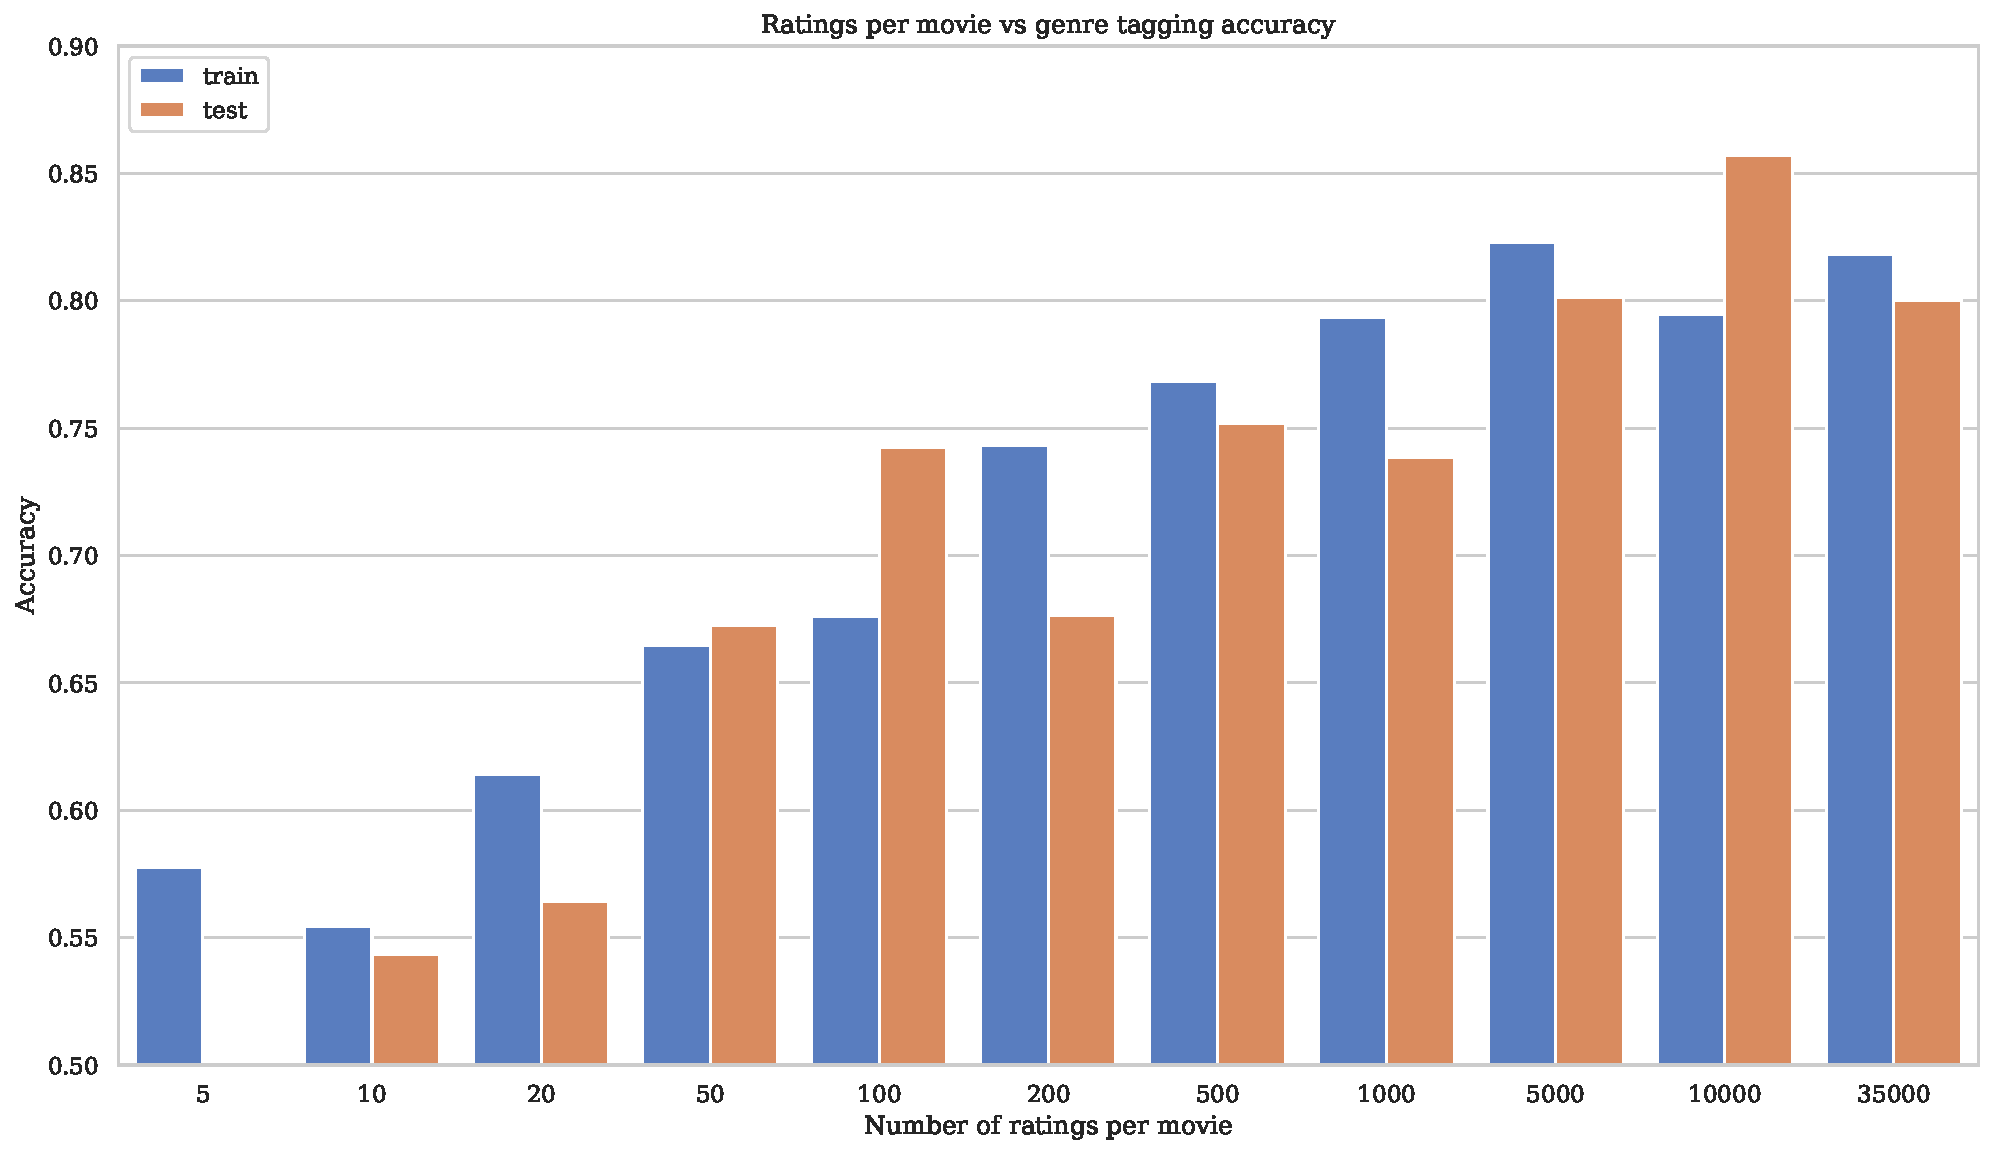
\includegraphics[width=0.85\textwidth]{Figures/5_ml10m-ratings-vs-acc.pdf}
\decoRule
\caption[Number of ratings vs accuracy]{Movies with more ratings tend to be more accurately classified.}
\label{fig:5-ratings-vs-acc}
\end{figure}

It can be seen in figure \ref{fig:5-ratings-vs-acc} that as the number of ratings per movie increases, the accuracy with which CGT can predict its genre increases too. For movies with 5000 or more ratings, the average classification accuracy is over 80\%.

\section{Latent factor analysis}
To understand the relationship between the latent factors in the embedding layer and genres in ML10M, the item embedding matrix was reduced from 200 dimensions to 2. Dimensionality reduction was done using principal component analysis, in which the 200-dimensional space of the embedding matrix was decomposed into 2 mutually orthogonal dimensions -- or components -- that captured the maximum amount of variance from the original space. While this reduction in dimensionality inevitably leads to a loss of information, it allows the movies to be visualised in the latent factor space.

\subsection{Distribution of genres}
Figure \ref{fig:5-genre-pca} shows the distribution of two genres, "Children" and "Documentary", in the first two principal components of the latent factor space. Out of the total 10 000 movies in ML10M, 528 are classified in the "Children" genre and 479 are documentaries. There are only 2 movies which are labelled as both a children's film and a documentary.

\begin{figure}[H]
\centering
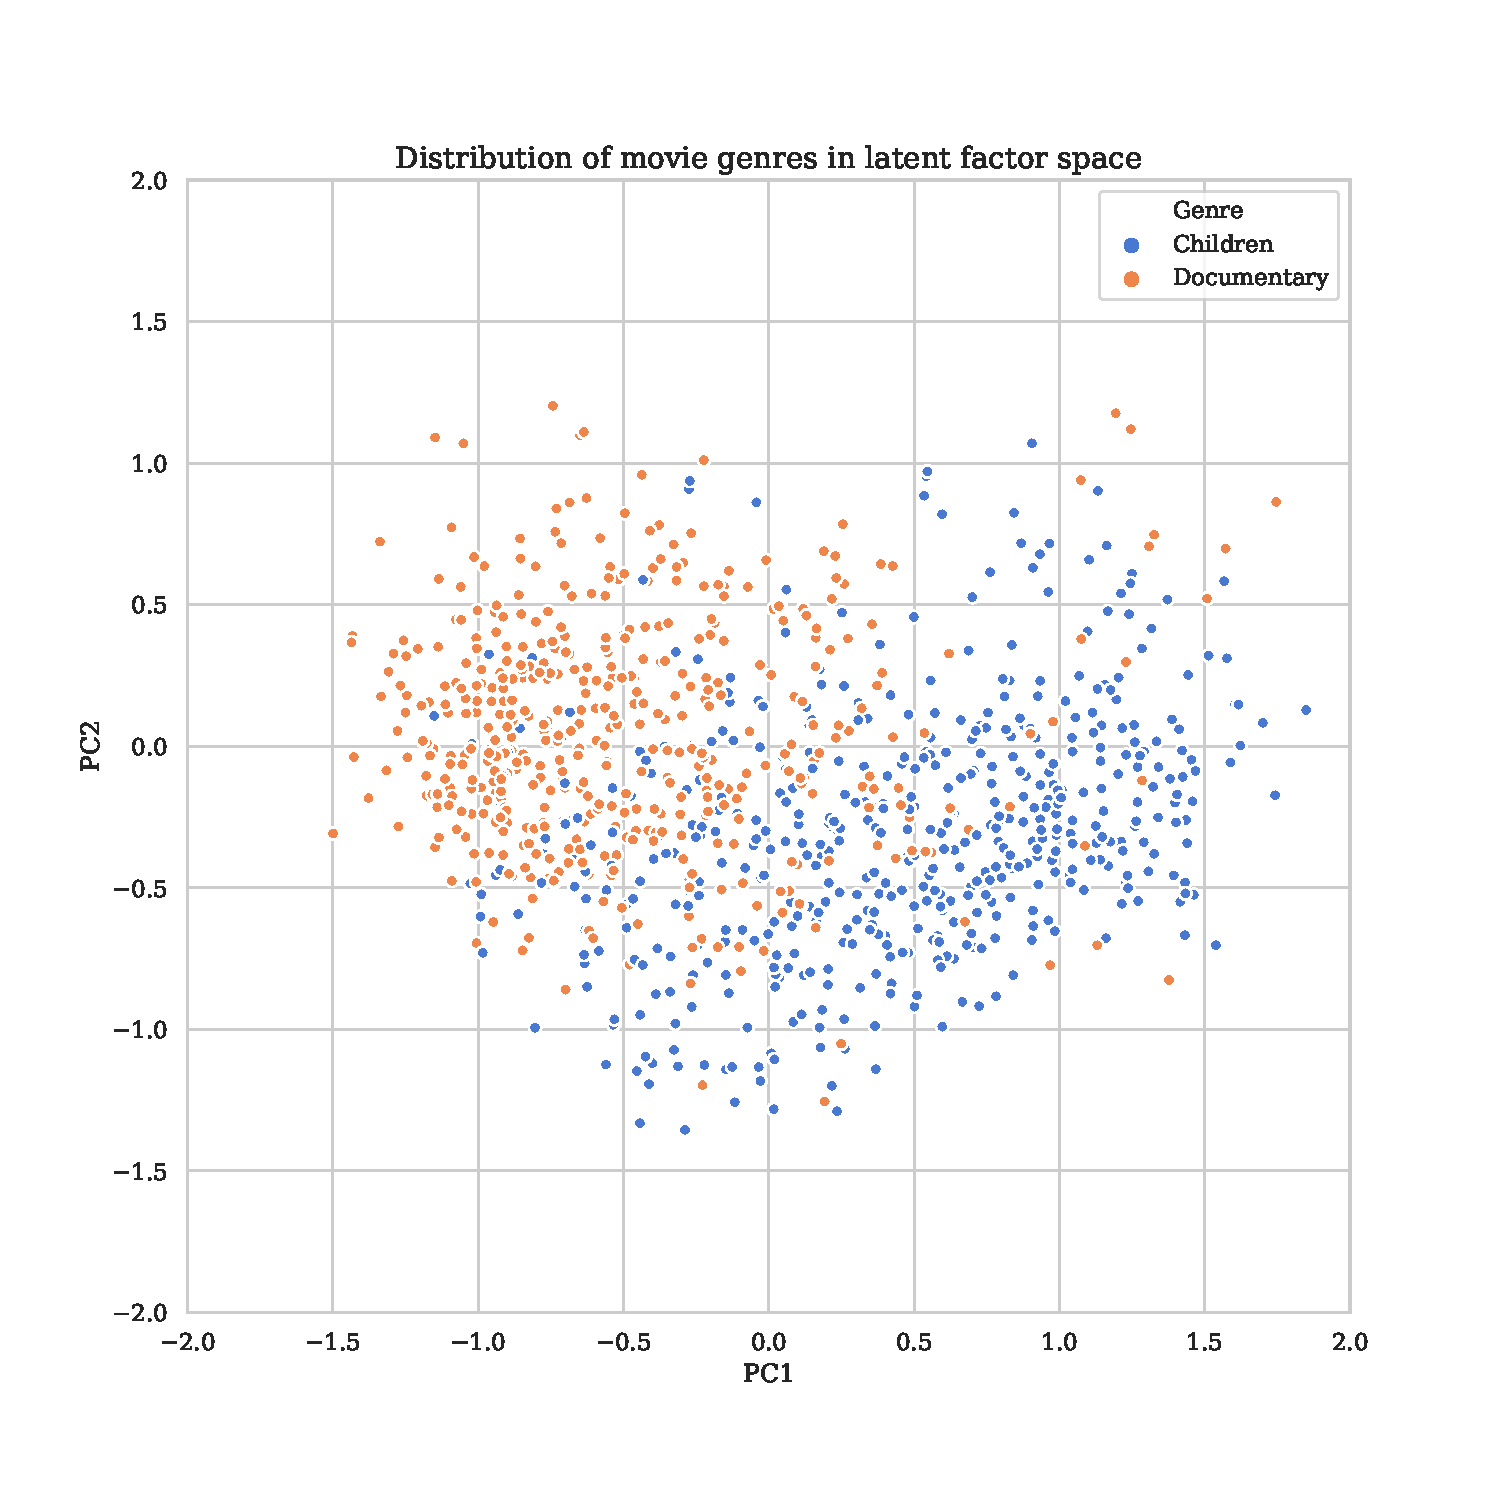
\includegraphics[width=0.7\textwidth]{Figures/5_ml10m-genre-pca.pdf}
\decoRule
\caption[Distribution of genres in latent factor space]{Children's movies and documentaries shown in the first two principal components of the latent factor space.}
\label{fig:5-genre-pca}
\end{figure}

Although the genre model was not trained to predict either of these genres, this figure serves to illustrate the inherent ability of the latent factors to capture descriptive features of movies. While not entirely separable, the difference in principal component loadings between these two genres can be seen in just two dimensions. The geometric means of each genre are given in table \ref{tab:ml10m-genre-pca}

\begin{table}[H]
\centering
\begin{tabular}{c | c | c}
\toprule
\textbf{Genre} & \textbf{$\Bar{PC1}$} & \textbf{$\Bar{PC2}$} \\
\midrule
Children & 0.437 & -0.300 \\
\midrule
Documentary & -0.477 & 0.046 \\
\bottomrule
\end{tabular}
\caption[Genre principal component means]{Geometric means of "Children" and "Documentary" genres in first two principal components of latent factor space.}
\label{tab:ml10m-genre-pca}
\end{table}

It is shown above that the centre of "Children" genre has a moderately strong positive loading in the first principal component, while the centre of the "Documentary" genre has a similarly strong negative loading.

\subsection{Distribution of ratings}
Figure \ref{fig:5-ratings-scatter} shows the 10 highest rated movies alongside the 10 lowest rated movies. There is a clear separation between these two groups.

\begin{figure}[H]
\centering
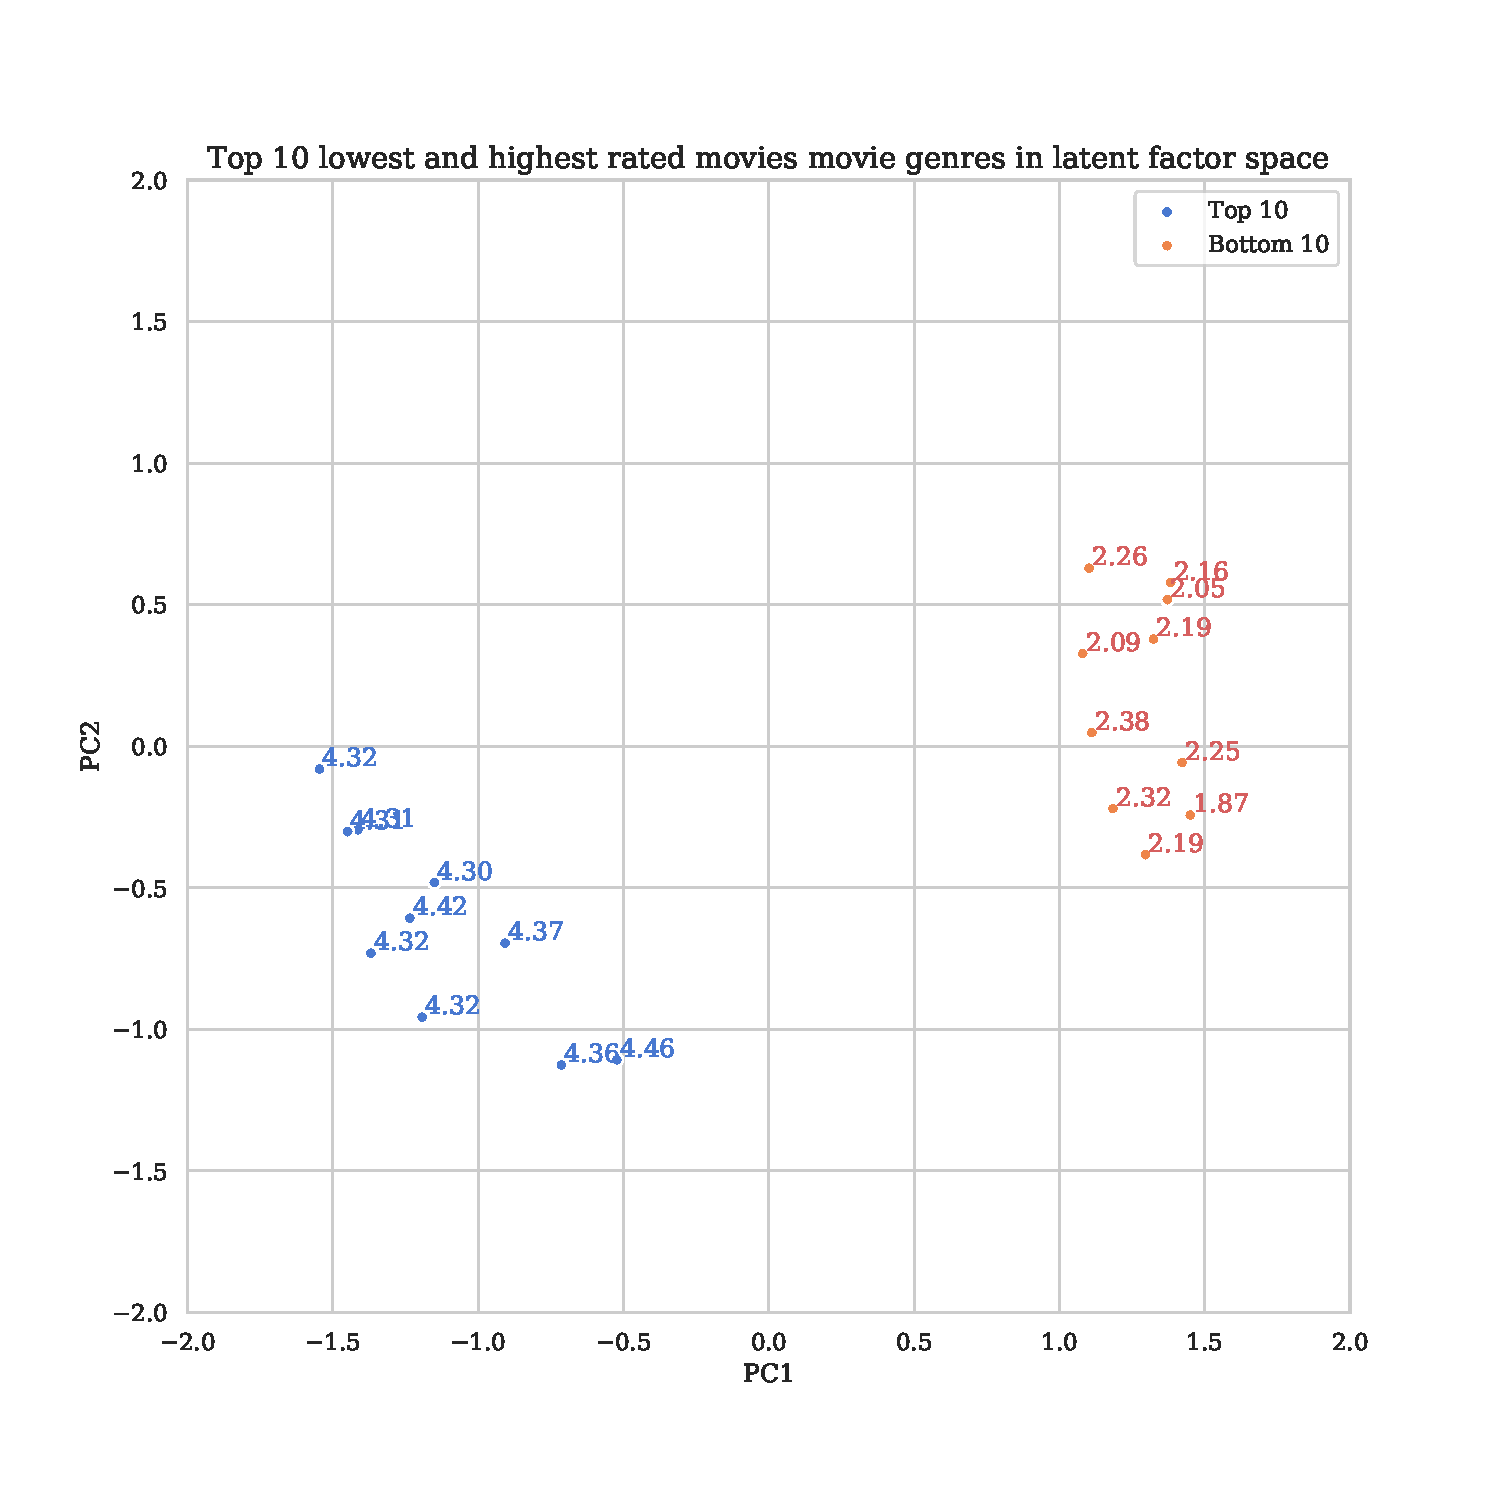
\includegraphics[width=0.69\textwidth]{Figures/5_ml10m-ratings-scatter.pdf}
\decoRule
\caption[Top 10 highest and lowest rated movies]{Top 10 highest (blue) and lowest (red) rated movies in first two principal components. Each point is annotated with its average user rating.}
\label{fig:5-ratings-scatter}
\end{figure}

The highest rated movies all have strong negative loadings in the first principal component, while the lowest rated movies all have equally strong positive loadings. Figure \ref{fig:5-ratings-hexbin} provides a visualisation of the average rating of all 10 000 movies in the latent factor space.

The 'hex bin' plot groups movies into hexagons, the boundaries of which are defined in PC1 and PC2. The value of each hexagon is calculated as the mean rating of all movies that fall inside its boundaries. There is a clear pattern of higher rated movies towards the bottom left of the coordinate grid, with the lowest rated movies in the top right.

\begin{figure}[H]
\centering
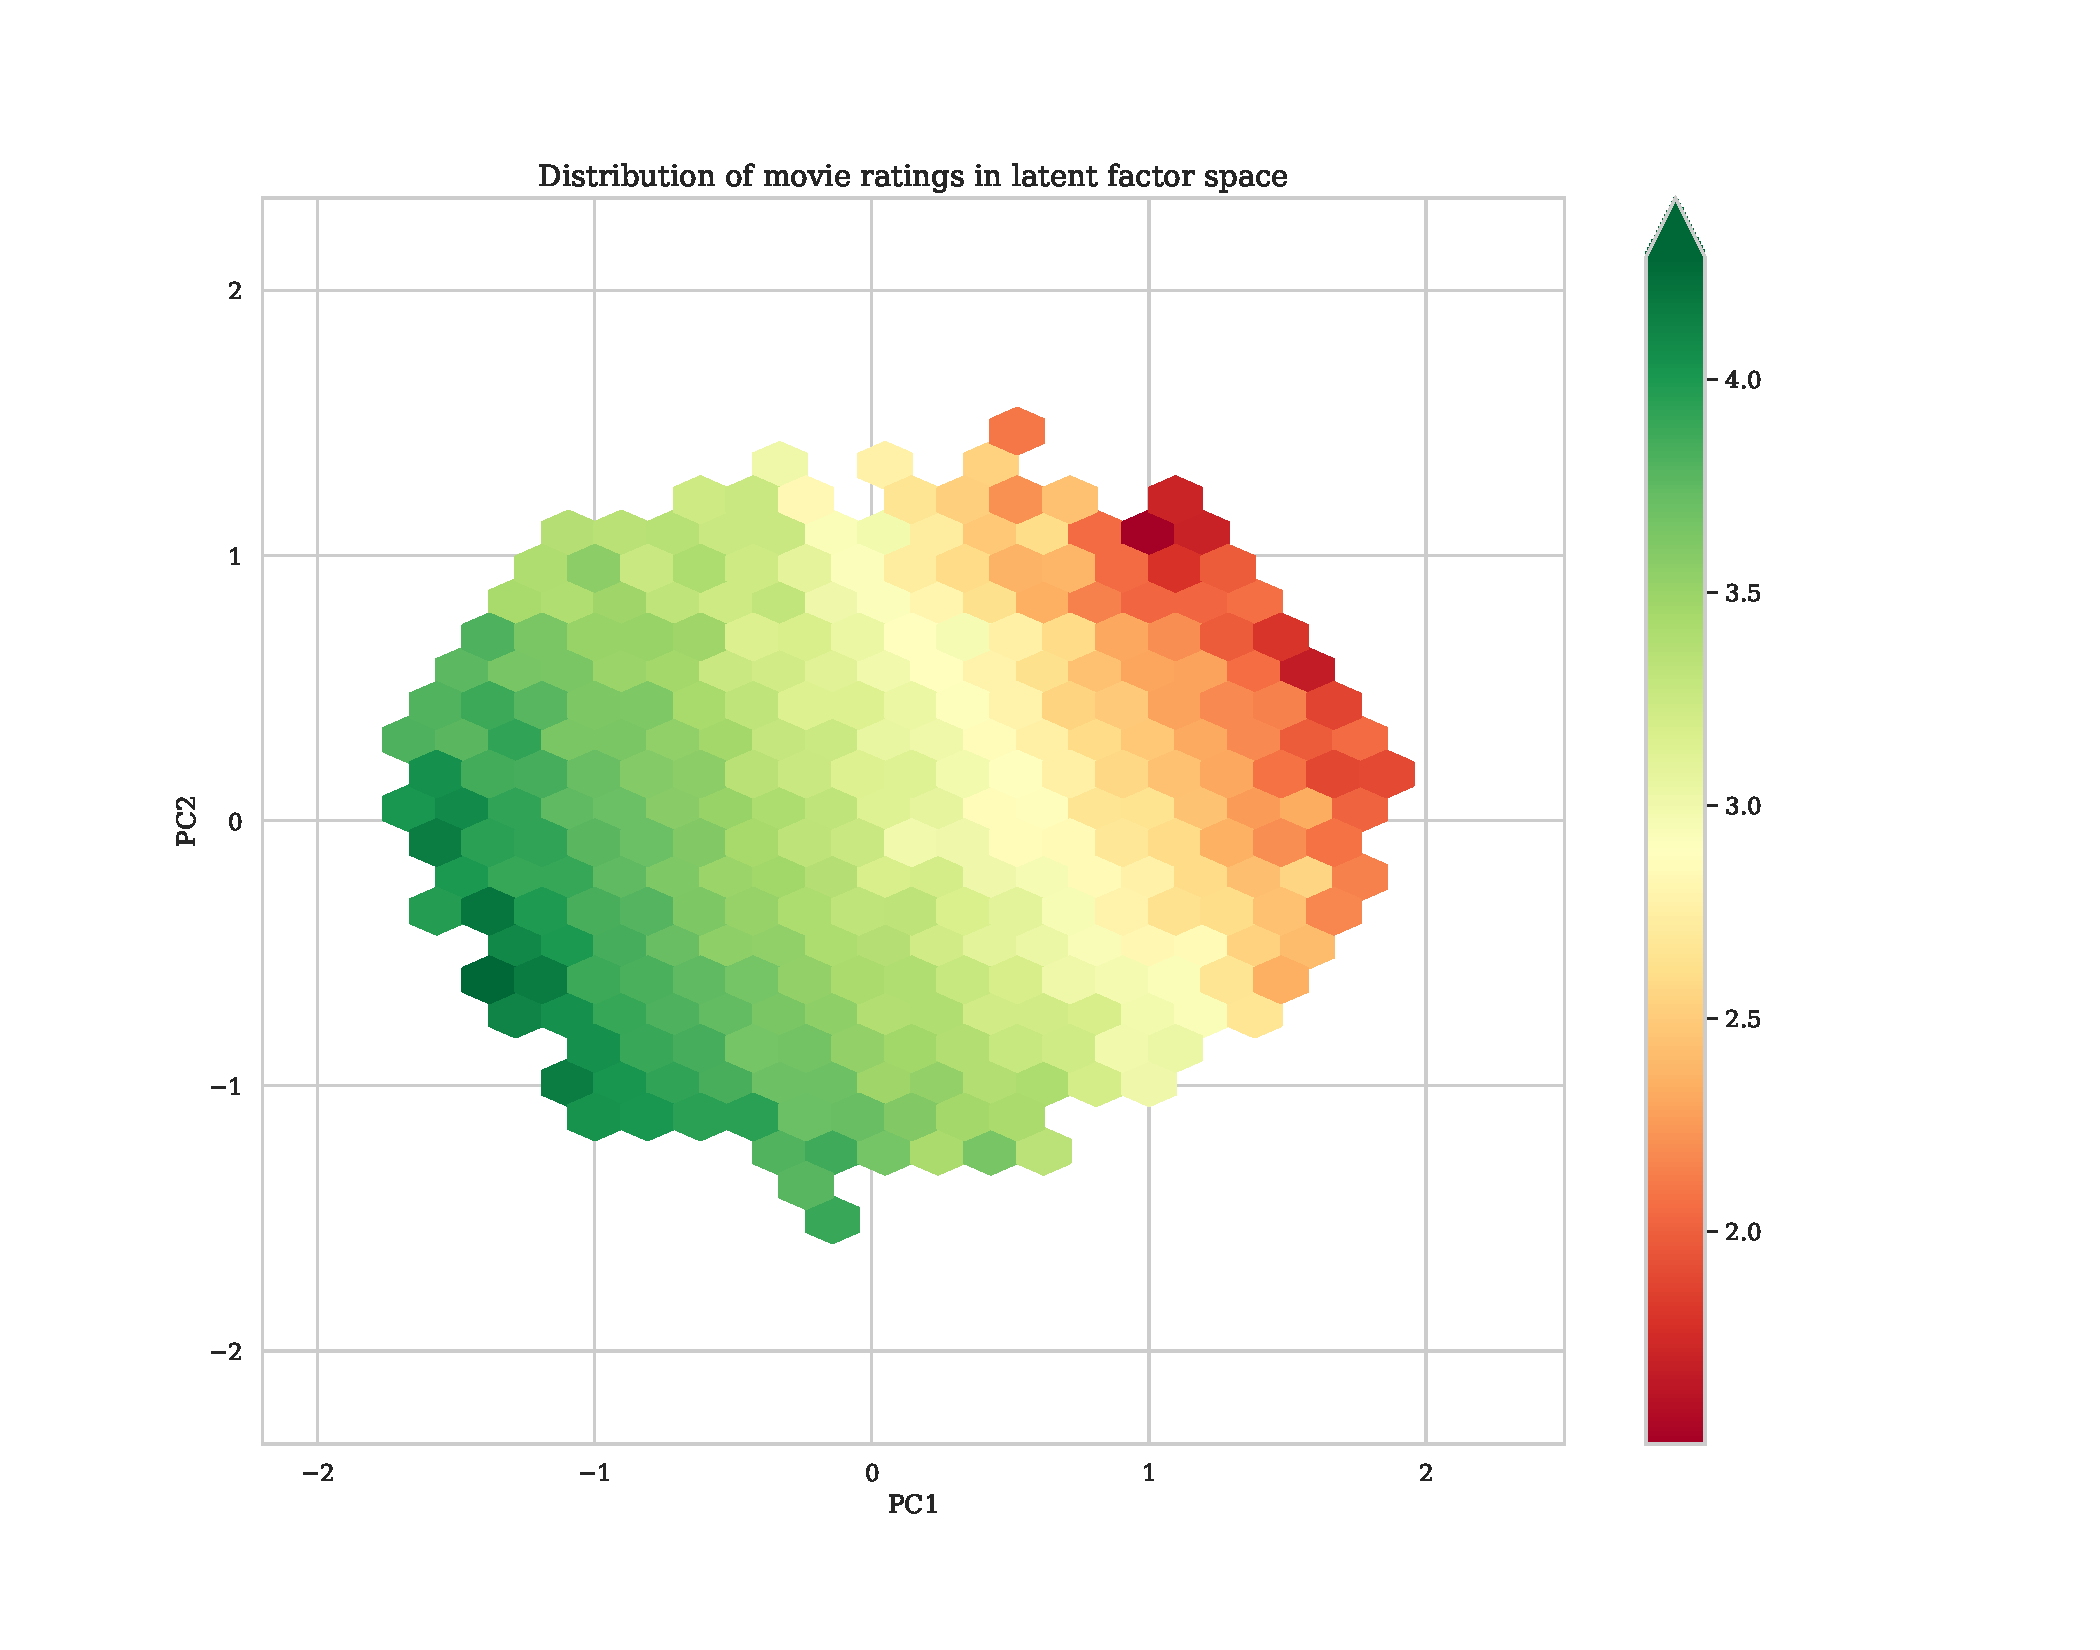
\includegraphics[width=0.74\textwidth]{Figures/5_ml10m-ratings-hexbin.pdf}
\decoRule
\caption[Average rating hex bin plot in PC1 and 2]{Hex bin plot shows average rating within each hexagon. Movies in the bottom left receive higher ratings on average than those in the top right.}
\label{fig:5-ratings-hexbin}
\end{figure}

\subsection{Classification accuracy}
Finally, the relationship between latent factors and classification accuracy was explored. A similar hex bin plot to figure \ref{fig:5-ratings-hexbin} was used, but instead showed the mean classification accuracy in each hexagon. This is shown in figure \ref{fig:5-accuracy-hexbin}.

Interesting to note is the higher accuracies observed at the more extreme loadings of PC1 and PC2. This suggests that movies with more extreme latent factor values are more descriptive and therefore possibly easier to predict. If this is indeed the case, then the goal of the rating model in CGT should be to train latent factors that are maximally dissimilar to each other.

\begin{figure}[H]
\centering
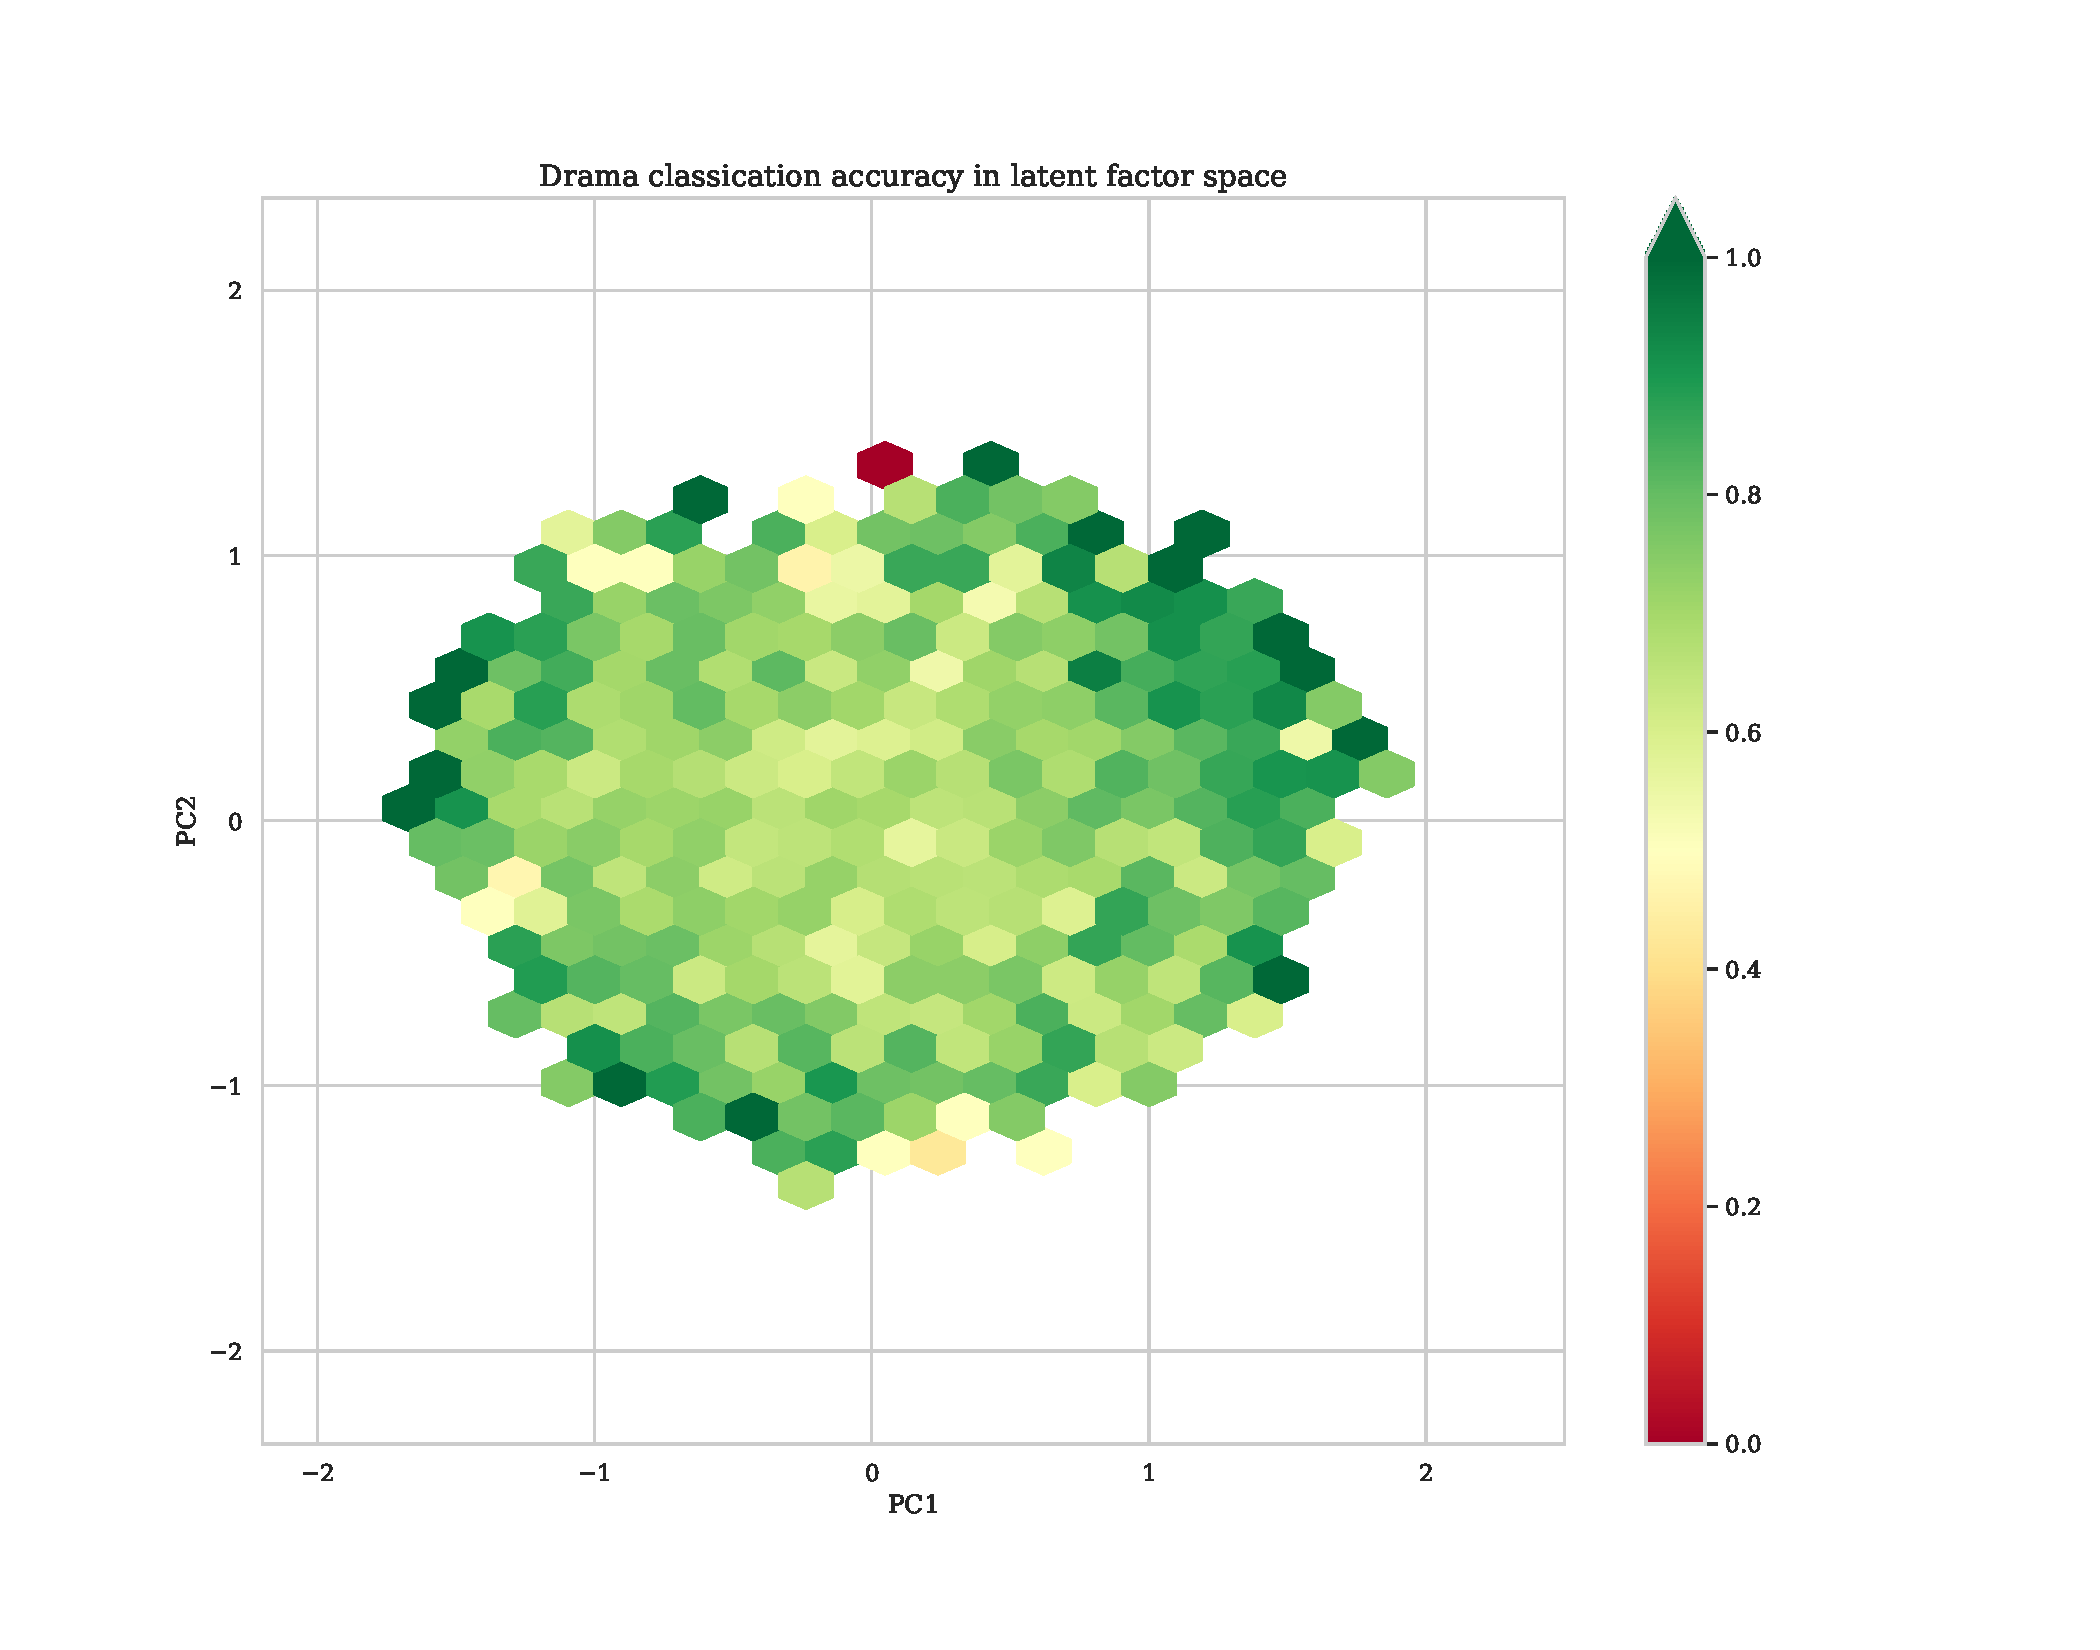
\includegraphics[width=0.74\textwidth]{Figures/5_ml10m-accuracy-hexbin.pdf}
\decoRule
\caption[Classification accuracy hex bin plot in PC1 and 2]{Classification accuracy across PC1 and PC2 of latent factor space. Movies with more extreme latent factors tend to have more extreme accuracy scores.}
\label{fig:5-accuracy-hexbin}
\end{figure}